\documentclass[a4paper,12pt]{article}
\usepackage[utf8]{inputenc}

% Larger borders -- we do not want do waste paper, even if it is only paper on screen =)
\usepackage[top=2.5cm, bottom=2.5cm, left=2cm, right=2cm]{geometry}

% No paragraph indentation
\setlength{\parindent}{0cm}

% Palatino font (nicer serif font: Times is for oldies)
\renewcommand*\rmdefault{ppl}

% Nested itemize list bullet style
\renewcommand{\labelitemi}{$\bullet$}
\renewcommand{\labelitemii}{$\circ$}
\renewcommand{\labelitemiii}{--}

% Math packages
\usepackage{amsmath}
\usepackage{amsfonts}
\usepackage{amssymb}

% Graphic packages
\usepackage{graphicx}
\usepackage{float}
\usepackage{adjustbox}
\usepackage{tikz}
\usepackage{forest,array}
\usetikzlibrary{shadows}

% Timing diagrams
\usepackage{tikz-timing}
\usetikztiminglibrary{arrows}

% Graphs styles
\forestset{
  giombatree/.style={
    for tree={
      grow = east,
      parent anchor=east,
      child anchor=west,
      edge={rounded corners=2mm},
      fill=violet!5,
      drop shadow,
      l sep=10mm,
      edge path={
        \noexpand\path [draw, \forestoption{edge}] (!u.parent anchor) -- +(5mm,0) -- (.child anchor)\forestoption{edge label};
      }
    }
  }
}
\forestset{
  qtree/.style={
    for tree={
      parent anchor=south,
      child anchor=north,
      align=center,
      edge={rounded corners=2mm},
      fill=violet!5,
      drop shadow,
      l sep=10mm,
    }
  }
}

% Hides ugly links from the index
\usepackage[hidelinks]{hyperref}

% Landscape format pdf pagess
\usepackage{pdflscape}

% Overline in text mode
\makeatletter
\newcommand*{\textoverline}[1]{$\overline{\hbox{#1}}\m@th$}
\makeatother

%%%%%%%%%%%%%%%%%%%%%%%%%%%%%%%%%%%%%%%%%%%%%%%%%%%%%%%%%%%%%%%%%%%%%%%%
% Specific commands for this document
\newcommand{\computername}{CA~19.32}
\newcommand{\memoryname}{Elephant}

% Title
\title{\memoryname{} DRAM}

% Authors
\author{G. Alvaro, F. Barbarulo, D. Comola, F. Fornaini, R. Polini, G.B. Rolandi}

\begin{document}
\maketitle
\tableofcontents

\clearpage

\section{Introduction}

This document describes the working details of the main memory and the main bus of the Computer~Architecture course computer.

\subsection{Bus}
Main bus is 16~bit wide address and 32~bit wide data bus.

\subsection{\memoryname{}}
\memoryname{} is a SDR DRAM, single data rate dynamic random access memory.

It can hold a total amount of 512~Kbit (64~KiB) of data, and can be accessed as 16~K locations of 32~bit (4 B) each.

\section{Main computer bus}
Physical main bus of \computername{} presents the following wires.

\begin{figure}[H]
\centering
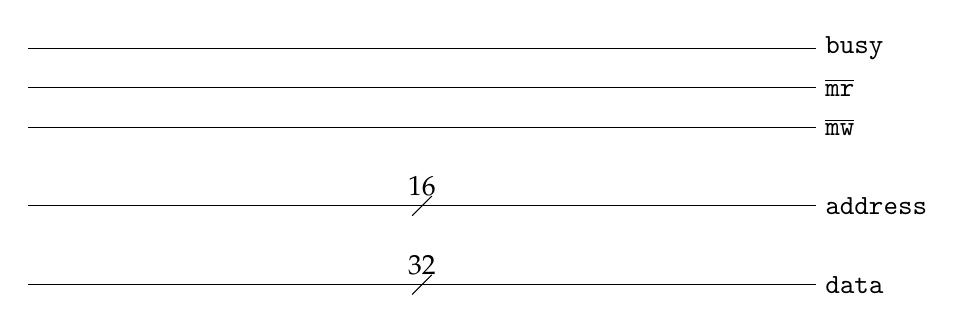
\begin{tikzpicture}
  % data wires
  \draw (0, 1)--(10, 1);
  \node at (5, 1){};
  \node [draw, strike out] at (5, 1){};
  \node [above] at (5, 1){32};
  \node [right] at (10, 1){\texttt{data}};

  % address wires
  \draw (0, 2)--(10, 2);
  \node at (5, 2){};
  \node [draw, strike out] at (5, 2){};
  \node [above] at (5, 2){16};
  \node [right] at (10, 2){\texttt{address}};

  % mw
  \draw (0, 3)--(10, 3);
  \node [right] at (10, 3){\textoverline{\texttt{mw}}};
  % mr
  \draw (0, 3.5)--(10, 3.5);
  \node [right] at (10, 3.5){\textoverline{\texttt{mr}}};

  % busy wire
  \draw (0, 4)--(10, 4);
  \node [right] at (10, 4){\texttt{busy}};
\end{tikzpicture}
\caption{main bus of \computername{}}
\end{figure}

% explanation
\begin{itemize}
  \item \textbf{busy:} this wire represents the busy status of the bus; the busy wire is active high.
  \item \textbf{\textoverline{mr}:} this wire issues a read data command, and instructs a module to put data from its internal structures onto the bus; the \textoverline{mr} wire is active low;
  \item \textbf{\textoverline{mw}:} this wire issues a write data command, and instructs a module to retrieve data from the bus and put into its internal structures; the \textoverline{mw} wire is active low;
  \item \textbf{address:} is 16~wires wide and selects the address from which/to which data must be read/written;
  \item \textbf{data:} is 32~wires wide and holds the actual data that must be read or written;
\end{itemize}

Thus, main computer bus can be represented in the simulation software by means of the following global \texttt{Bus} structure.

\begin{verbatim}
struct Bus {
  bool busy;
  bool _mr, _mw;
  uint16_t address;
  uint32_t data;
}
\end{verbatim}

% BHA Protocol
\subsection{Bus handshake protocol}
In the simulation software, modules can:
\begin{itemize}
  \item be idle: this corresponds to the high impedance physical state;
  \item perform a read action from the bus;
  \item perform a write action on the bus;
\end{itemize}

Actions on bus must be performed in the simulation using the following protocol.

\begin{itemize}
  \item being idle: \texttt{bus} structure must not be read or written;
  \item read data: data can be read only upon receiving a message from another module.
  When data has been read from the global \texttt{bus} structure into local structures, bus busy bit must be clear to terminate the handshake.
  \item write data: when a module wants to occupy the bus for writing data, first it must ensure that bus is free by checking the busy wire status.
  \begin{itemize}
    \item if busy bit is 0, data can be written onto the bus and bus busy bit must be set; moreover, destination module must be notified of the bus change by sending it a message using methods provided by the orchestrator.
    For the sake of simplicity, message passed through the orchestrator can be tought as a model for the hardware \emph{enable} wire;
    \item if busy bit is 1, data must not be written onto the bus, and module must wait for the next quantum of time (\emph{tick});
  \end{itemize}
\end{itemize}

Please note that this does not model the actual hardware behavior, since a reading module can not clear a set bit on the bus; but since it is not necessary to perfectly reproduce the hardware behavior, this handshake is used in order to simplify the simulation software.

Note: since simulation is sequential and modules are always notified in the same order, concurrency is not actually modeled, and some modules can suffer from starvation.

% thus, a proper read/write operation can be represented in time like the following timing diagram:
% busy
% mr
% mw
% address
% data
% (be careful and remember to represent both the read and the write operation examples)

% TO BE DONE
\begin{figure}[H]
\centering
\begin{tikztimingtable}
{busy}              & D{0}  2D{1} D{0}\\
{\textoverline{mr}} & X     2D{0} X\\
{\textoverline{mw}} & X     2D{1} X      \\
{address}           & X     2D{}  X\\
{data}              & X     2X    D{}\\
\\
{send event}        & L     L A   L\\
%~ \extracode
%~ \begin{tikzpicture}
  %~ \foreach \x in {1,...,6}
  %~ \draw (\x,-7)--(\x,0);
%~ \end{tikzpicture}
\end{tikztimingtable}
\caption{read handshake}
\end{figure}

\section{DRAM Internals}
\subsection{Circuit}
% proper picture of our dram
% with cell matrix

\subsection{Input and output}
% all I/O lines and their description:
% /ras
% /cas
% Address
% R/W
% data

\section{DRAM control}
\subsection{Simple read/write}
% timing diagram
\subsection{Fast page read/write}
% timing diagram

\section{Timings definition}
% t_CL  CAS latency
% t_RCD row address to column address delay
% t_RP  row precharge time
% t_RAS number of clock cycles to refresh a row

% and their description

\section{Interesting cases}
% accessing a bit from a DRAM with the right row open (CL)
% accessing a bit from a DRAM without an active row (t_RCD + t_CL)
% accessing a bit from a DRAM with the wrong row open (t_RP + t_RCD + t_CL)

\section{Test}
% test

\section{Transfer speed}
Since this is a \emph{single data rate} memory, in short SDR, it is theoretically possible to read or write data from/to the memory once for every rising edge of the bus clock.

Thus, maximum theoretical transfer speed is given by the following formula:

$$ s_{max} =  f \cdot B_w $$

where

\bgroup
\def\arraystretch{1.5}
\begin{table}[H]
\center
\begin{tabular}{| c | c | c |}\hline
\textbf{symbol} & \textbf{unit} & \textbf{description} \\ \hline
$ s_{max} $ & $ \frac{bit}{s} $ & maximum theoretical speed \\ \hline
$ f $ & Hz & bus frequency \\ \hline
$ B_{w} $ & bit & bus width \\ \hline
\end{tabular}
\end{table}
\egroup

\section{EOF}
This is the End of File.

\end{document}
